\documentclass[a4paper, 12pt]{exam}

\usepackage[onehalfspacing]{setspace}
\usepackage{graphicx}
\usepackage{amsmath,amsfonts,amsthm,amssymb,mathtools}
\usepackage{nameref}
\usepackage{hyperref}
\usepackage{xcolor}
\usepackage{gensymb}
\usepackage[]{booktabs}
\usepackage[utf8]{inputenc}
\usepackage{array}
\usepackage{setspace}
\usepackage{verbatim} %for multiline comments https://tex.stackexchange.com/questions/44282/multiline-comment
\usepackage{xhfill}
\usepackage{enumitem}
\usepackage{varwidth}
\usepackage{multicol, array}
\usepackage{etoolbox}
\usepackage{multicol}
\usepackage[most,many,breakable]{tcolorbox}
\usepackage{mathtools}
\usepackage{background} %Package for adding a watermark
\usepackage{tikz-cd}
\usepackage{pgfplots} 
\pgfplotsset{compat=newest}
\usepgfplotslibrary{patchplots}
\usepackage{anyfontsize}
\usepackage{sectsty}
\usepackage[space]{grffile} %To allow for spaces in the path for the watermark
\usepackage{amsmath}
\usepackage{geometry} %lets us set the margins of the page
\usepackage{comment} %Allows for multi-line comments (\ifx \fi)
\usepackage{import} %lets us perform multi-file compilation
\usepackage{pdfpages} %allows for the inclusion of external multi-page PDF documents
\usepackage{algpseudocode} %lets you write algorithms (probably won't be used but i'm including it anyways) https://www.overleaf.com/learn/latex/Algorithms
\usepackage{bookmark}
\usepackage{theorem}

\geometry{left=0.8in,top=0.5in, right = 0.8in}

\newcommand{\cuspac}{\hspace*{1cm}}

\backgroundsetup{contents=
\includegraphics{Anant_Logo.png}, opacity=0.1, angle=0, scale=1.5}

\begin{document}
	\title{Anant 24-25 Recruitment Test}
	\author{Attitude Determination and Controls Subsystem (ADCS)}
	\date{January 12th, 2024}
	\maketitle
	
	\section*{Instructions}
	All general instructions are provided in the Google Classroom. Make sure you refer to them for submission details. Failure to adhere to the given rules may result in disqualification. 
	\begin{enumerate}[]
		\item This paper relies more on comprehension and general aptitude than it does in depth knowledge of the subject. You are encouraged to use the internet to solve this paper.
		\item Any changes to the paper will be posted in Google Classroom and an updated file will be shared. Please keep an eye out.
	\end{enumerate}
	Rules of engagement
	\begin{enumerate}[label = \textbf{Rule \arabic* }:, leftmargin=5em]
		\item A student must prioritize developing an understanding of the topics being tested and demonstrating general aptitude, as evaluated during the subsequent interview where their solutions will be the main topic of discussion.
		
		\item A student must not collaborate with peers unless such collaboration is necessary to better achieve the goals outlined in Rule 1.
		
		\item A student must prioritize their physical and mental well-being, avoiding undue stress, all-nighters, or harmful study practices, unless doing so would conflict with Rules 1 or 2.
		\item If you have any questions regarding the content of the paper, feel free to reach out to any of the undersigned through WhatsApp for help. (Do not call)
		\item Contact Details:
		\begin{enumerate}
			\item Aaditya Thakkar - +91 81282 17114
			\item Nikhil Mathew - +91 97400 44411 (Most helpful you can call him)
			\item Pranav Chandra - +91 90807 96426
			\item Pramit Pal - +91 99026 97222
		\end{enumerate}
	\end{enumerate}
	\begin{center}
		All the best!
	\end{center}
		
	\pagebreak
	
	\newgeometry{left=1in,top=1.25in, right = 1in}
	
	\section*{}
	

	\section*{Question 1 - Bob's Search for the Hill of Happiness}
	Bob, in his insanity of life, is looking for a mountain, Korok, which claims to have the best weed in the world. However, to find it, he must first decode a map, and achieve his state of high.
	
	\begin{enumerate}[label=(\alph*)]
		\item The map was created by a sadistic being at 13:00 GMT on the 2nd of January, 1920 in honor of a great man born on that day. He used what us mortals now call the \textit{Fixed Frame}, which is defined as follows:
		\begin{center}
			\textit{The origin is the center of the Earth. The positive z-axis is the ray passing through the geographic north pole of the earth. The positive x-axis is in the direction of the vernal equinox, and the y-axis is taken as the right-hand cross product of the x and z axes.}
		\end{center}
		The coordinates in the map are $(3580.20,1105.36,5152.67)$ in \textit{km}. Convert these coordinates into latitude-longitude-altitude to find out where the hill is. In your answers, include sketches of both the Fixed Frame and the Latitude Longitude frame, as well as a marking of points. (Assume, \textbf{for the sake of the question,} that the x-axis of the\textit{ Fixed Frame} passes through the intersection of the prime meridian and the equator every 24 hours at 12:00 GMT).
		
		\item Bob is way too far away from this point to get to on foot, so he'll be using his teleporter. However, his teleporter requires \textit{Rotating Frame} coordinates, defined as follows:
		\begin{center}
			\textit{The origin is the center of the Earth, and the x-axis is in the direction of the intersection between the prime meridian and the equator from the center of the earth. The y-axis is the left-hand cross product of the x and z axes.}
		\end{center}
		Convert the latitude-longitude-altitude coordinates from the previous part into the \textit{Rotating Earth} frame. Now, if you were unable to complete the first part of this question, that's alright. The higher beings have decided to give you the latitude-longitude-altitude to a Hill of Slightly-Less-Happiness  $(28\degree21'12.8"N 75\degree35'36.7"E)$, which Bob is okay with. 
		
		\pagebreak
		
		\item Unfortunately, bob is now stranded in outer space because his teleporter actually works with the \textit{Sun Fixed Frame}, defined as follows:
		\begin{center}
			\textit{The z-axis passes through the center of the sun and is perpendicular to the orbital plane. The x-axis is in the direction of the vernal equinox passing through the center of the sun. and the y-axis is the cross product of the x and z axes.}
		\end{center}
		He is now \textit{inside the sun}. Given that today is the 17th of January, 2025, find out the new coordinates he should teleport to in order to make it back to orbit around the earth at an altitude of $200km$. \href{https://ssd.jpl.nasa.gov/horizons/app.html#/}{Hint}
		
		\item Now that Bob is orbiting earth at an altitude of $200km$ sketch his reference frame so that the $x-axis$ is pointing down towards the earth and the $z-axis$ is in the direction of the orbit. Draw the orbit as well. 
		
		[Bonus] Find out how fast he has to spin in order for his eyes to continually point towards earth as he orbits.
	\end{enumerate}
	
	\pagebreak
	
	\section*{Question 2 - Bob's Fever Dream}
	Now that the weed has entered Bob's system, he's drifted into another plane. He's spiralling off of earth's surface and is now in an orbit with an altitude of $200km$. However, he wants to settle into an orbit at an altitude of $4206km$, using the least amount of energy. With his tiny rocket, he can only apply a burn of any impulse at three points in time. Find out the orbital transition and draw a diagram of where the burns should be made, and how much impulse should be provided. Hint:
	
	\begin{figure}[h!]
		\centering
		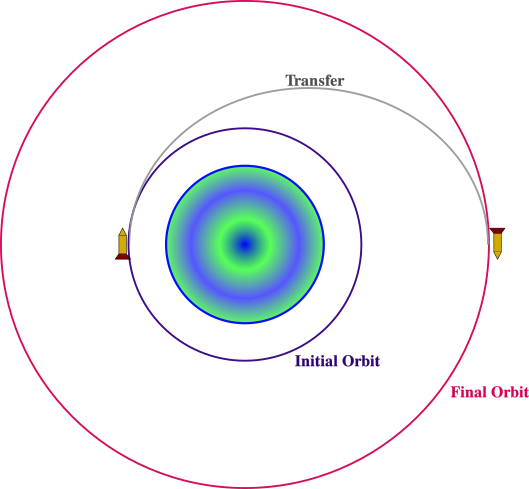
\includegraphics[scale = 0.8]{Q2_Transfer_Image.png}
	\end{figure}
	
	\pagebreak
	
	\section*{Question 3 - Trying to get back Home}
	Morty has now unfortuantely gotten separated from Rick in his travel through space. Before he got lost though, Rick gave him a GPS tracker. Although it's a little messed up because of his previous adventures, Morty is able to ping satellites and see the amount of time it takes for the signal to go from Morty to the satellite and back. 
	
	Rick however, is a little f*****. He's only given Morty 3 of the four satellite positions relative to him. They are:
	\begin{align*}
		A = \{-3141, -5926, 5358\}\\
		B = \{-9793, 2384, -6264\}\\
		C = \{3383, -2795, -288\}
	\end{align*}
	\begin{enumerate}[label = (\alph*)]
		\item Morty's first job is to figure out where the fourth satellite is. He knows Rick is enough of an a**h*** to make sure that none of the satellites are in the same octant. He also knows that the $x$, $y$ and $z$ coordinates of the satellite are probably the same. Find the position of the fourth satellite.
		\item Congratulations on finding the fourth satellite, unfortunately Morty pressed the button labelled don't press, setting off a hidden rocket inside the GPS has suddenly gone off, sending Morty tumbling through the universe. Before the GPS dies, Morty gets two sets of pings off the satellites.
		\begin{align*}
			A_1 = 28.21941442 ms \cuspac A_2 = 32.56521822 ms\\
			B_1 = 37.40539321 ms \cuspac B_2 = 37.48077648 ms\\
			C_1 = 21.88477974 ms \cuspac C_2 = 35.47581482 ms\\
			D_1 = 7.603382343 ms \cuspac D_2 = 21.38749482 ms
		\end{align*}
		\begin{enumerate}[label = (\roman*)]
			\item According to the clock, the first ping is at $t_1 = 0$ seconds, and the second is at $t_2 = 5000$ seconds (Rick is a b****). Find the direction vector and the velocity of Morty as he hurtles through space trying not to c*** his pants.
			\item Turns out, the second ping was actually sent at time $t_2 = 0.1$ seconds. Write down some of your favorite curse words to throw at Rick, and give us the direction vector and velocity of Morty.
		\end{enumerate}
		\item Morty has now landed in the orbit of Earth. His GPS splits into two pieces, a sun-sensor and a magnetic field sensor. Rick being Rick has also included a radio for Morty's use. However, for it to work, Morty needs to figure out his relative orientation to the planet. He bravely tapes the sensors to his chest pointing out, and he resigns himself to this horrible fate. Draw an approximate diagram with Morty, and show how he'd aptly describe his orienation to ground control.
	\end{enumerate}

	
	\pagebreak
	\section*{Question 4 - Bob's Cat}
	His cat has suddenly joined him. Measurements are taken every 0.5 seconds.
	\begin{enumerate}[label = (\alph*)]
		\item Given the first $n$ positions ${(x_1, y_1), (x_2, y_2), ... , (x_n, y_n)}$, estimate the true position of the cat.
		\item Obviously, noting down every position and finding the exact position every time is unfeasible (because data, duh). Give us a new expression that uses the $(n-1)_{th}$ estimation and the $n_{th}$ measurement to estimate the true position of the cat.
		\item If the measurements for the first 5 seconds are:
		\begin{equation*}
			1,2,3,4,5
		\end{equation*}
	\end{enumerate}
	
	
\end{document}